\section{The algorithm} \label{sec:algorithm}

\subsection{The data segmentation} \label{sec:algorithm:segmentation}

\subsection{The data access} \label{sec:algorithm:data}

\begin{figure}
  \center
  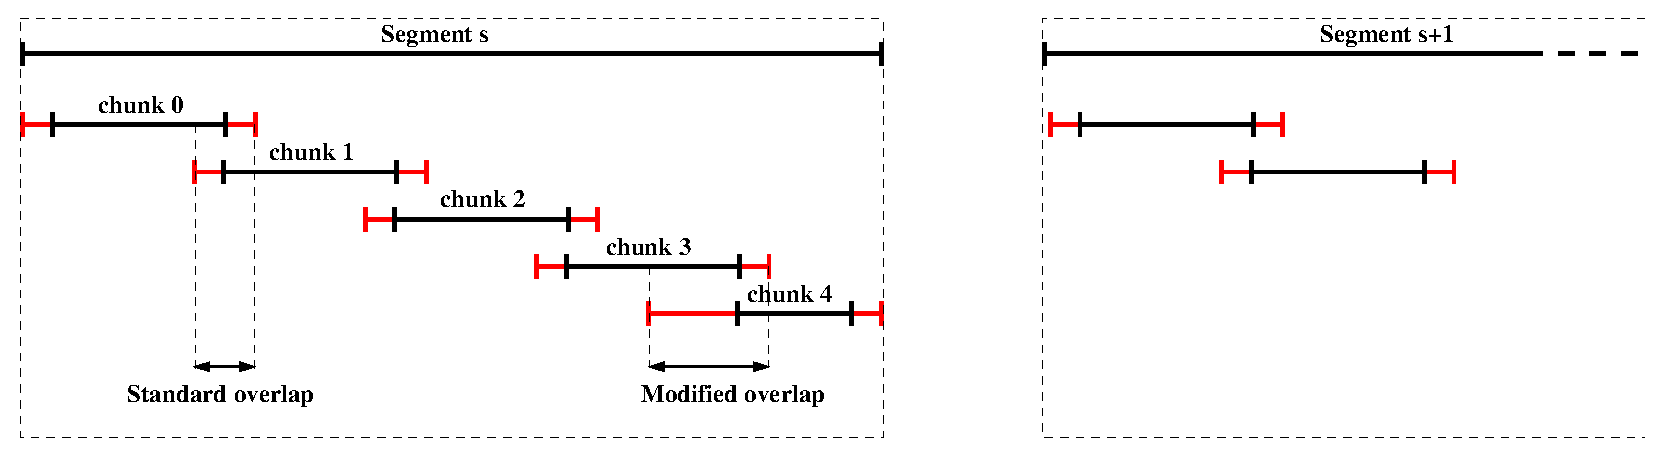
\epsfig{width=15cm, file=./figures/segmentation.eps}
  \caption{Data segmentation. The data are loaded by chunks and chunks are divided in blocks. The chunks have a duration $T$ and are used to estimate the power spectral density. The blocks have a duration $t$ and are analyzed sequentially. Chunks (and blocks) overlap with a duration $o$. This segmentation must therefore verify $T=n(t-o)+o$ where $n$ is an integer.}
  \label{fig:segmentation}
\end{figure}

\subsection{The power spectral density} \label{sec:algorithm:psd}

\subsection{The data conditioning} \label{sec:algorithm:conditioning}

\subsection{The tiling} \label{sec:algorithm:tiling}

\subsection{The filtering} \label{sec:algorithm:conditioning}

\subsection{The triggering} \label{sec:algorithm:triggering}

\subsection{The clustering} \label{sec:algorithm:conditioning}

\subsection{The mapping} \label{sec:algorithm:mapping}
